\section{Auswertung}
\label{sec:Auswertung}  

\subsection{Überprüfung der Aussagekraft der Messwerte}
\label{sec:Überprüfung}
Die Messwerte für die Spannungen von $\SI{150}{\volt}$, $\SI{170}{\volt}$, $\SI{190}{\volt}$, $\SI{210}{\volt}$
und $\SI{240}{\volt}$ sind \autoref{tab:t12}, \autoref{tab:t34} und \autoref{tab:t5} zu finden. Die gemessenen  
Thermistorwiderstände sind im Bereich von $\SI{1,895}{\mega\ohm}$ bis $\SI{1,922}{\mega\ohm}$, so dass nach der
im Anhang angegeben \autoref{fig:thermistor} für Thermistorwiderstände die
Temperatur zu $T\approx \SI{27}{\celsius} = \SI{301,5}{\kelvin}$ ablesbar ist. Es wurden nur Tröpfchen untersucht,
die keine Geschwindigkeit ohne angelegtes E-Feld haben, so dass die Messung von $t_{\symup{0}}$ nicht notwendig
ist. Die einzige Bewegung die die Tröpfchen aufgewiesen haben lässt sich durch die Brownsche Molekülbewegung
erklären und ist für $v_{\symup{0}}$ nicht von Relevanz, so dass sich für alle Tröpfchen
$v_{\symup{0}} = \SI{0}{\milli\meter\per\second}$ ergibt.
\begin{table}
  \centering
  \caption{Messwerte für $U=\SI{150}{\volt}$ und
  $U=\SI{170}{\volt}$.}
  \label{tab:t12}
  \begin{tabular}{c c c}
    \toprule
    Tröpfchen & $t_{\symup{ab}}/\unit{\second}$ & $t_{\symup{auf}}/\unit{\second}$ \\
    \midrule
    1 & 5,50 & 6,84 \\
      & 5,89 & 7,35 \\
      & 5,54 & 5,70 \\
    2 & 3,89 & 3,71 \\
      & 3,13 & 3,87 \\
      & 3,86 & 5,21 \\
    3 & 2,32 & 2,72 \\
      & 2,99 & 1,81 \\
      & 2,35 & 2,91 \\
    4 & 3,72 & 4,98 \\
      & 4,40 & 5,16 \\
      & 4,14 & 5,14 \\
    5 & 5,68 & 6,26 \\
      & 5,58 & 5,96 \\
      & 5,37 & 5,72 \\
    \bottomrule
  \end{tabular}
  \quad
  \begin{tabular}{c c c}
    \toprule
    Tröpfchen & $t_{\symup{ab}}/\unit{\second}$ & $t_{\symup{auf}}/\unit{\second}$ \\
    \midrule
    1 & 3,05 &  3,70 \\
      & 3,66 &  3,63 \\
      & 3,40 &  3,55 \\
    2 & 3,02 &  2,42 \\
      & 2,41 &  3,32 \\
      & 2,31 &  2,71 \\
    3 & 3,59 & 10,57 \\
      & 4,14 & 11,45 \\
      & 4,28 & 10,04 \\
    4 & 3,80 &  5,90 \\
      & 3,81 &  5,95 \\
      & 3,62 &  5,76 \\
    5 & 4,15 &  4,90 \\
      & 4,34 &  4,83 \\
      & 4,21 &  4,79 \\
    \bottomrule
  \end{tabular}
\end{table}

\begin{table}
  \centering
  \caption{Messwerte für $U=\SI{190}{\volt}$ und
  $U=\SI{210}{\volt}$.}
  \label{tab:t34}
  \begin{tabular}{c c c}
    \toprule
    Tröpfchen & $t_{\symup{ab}}/\unit{\second}$ & $t_{\symup{auf}}/\unit{\second}$ \\
    \midrule
    1 & 2,37 &  1,52 \\
      & 1,97 &  2,02 \\
      & 1,95 &  2,13 \\
    2 & 2,19 &  2,67 \\
      & 2,25 &  2,44 \\
      & 2,31 &  1,64 \\
    3 & 4,53 &  4,44 \\
      & 4,53 &  4,88 \\
      & 3,81 &  4,53 \\
    4 & 2,87 &  2,76 \\
      & 2,67 &  2,99 \\
      & 2,47 &  2,61 \\
    5 & 9,11 & 12,91 \\
      & 6,39 &  7,30  \\
      & 5,07 &  6,50  \\
    \bottomrule
  \end{tabular}
  \quad
  \begin{tabular}{c c c}
    \toprule
    Tröpfchen & $t_{\symup{ab}}/\unit{\second}$ & $t_{\symup{auf}}/\unit{\second}$ \\
    \midrule
    1 & 3,30 & 3,41 \\
      & 2,80 & 3,28 \\
      & 3,36 & 3,48 \\
    2 & 2,04 & 2,37 \\
      & 2,25 & 2,25 \\
      & 2,19 & 2,03 \\
    3 & 3,66 & 5,19 \\
      & 3,53 & 5,09 \\
      & 3,50 & 4,81 \\
    4 & 4,80 & 3,34 \\
      & 3,64 & 3,63 \\
      & 3,72 & 3,88 \\
    5 & 2,13 & 1,03 \\
      & 1,31 & 1,56 \\
      & 1,60 & 1,81 \\
    \bottomrule
  \end{tabular}
\end{table}

\begin{table}
  \centering
  \caption{Messwerte für $U=\SI{240}{\volt}$.}
  \label{tab:t5}
  \begin{tabular}{c c c}
    \toprule
    Tröpfchen & $t_{\symup{ab}}/\unit{\second}$ & $t_{\symup{auf}}/\unit{\second}$ \\
    \midrule
    1 & 1,75 & 1,95 \\
      & 2,24 & 2,14 \\
      & 2,35 & 2,51 \\
    2 & 2,33 & 6,03 \\
      & 3,66 & 5,51 \\
      & 3,19 & 6,22 \\
    3 & 1,78 & 1,25 \\
      & 1,35 & 1,57 \\
      & 1,88 & 1,61 \\
    4 & 1,79 & 2,19 \\
      & 1,79 & 1,95 \\
      & 2,19 & 2,40 \\
    5 & 2,24 & 2,75 \\
      & 2,36 & 2,79 \\
      & 2,46 & 2,77 \\
    \bottomrule
  \end{tabular}
\end{table}
Die Tröpfchen haben bei den gemessenen Zeiten einen Abstand von $s=\SI{0,5}{\milli\meter} = \SI{0,05}{\centi\meter}$
zurückgelegt, so dass sich aus den $t_{\symup{ab}}$ und $t_{\symup{auf}}$ die Geschwindigkeiten $v_{\symup{ab}}$ und
$v_{\symup{auf}}$ bestimmen lassen. Um sicher zu stellen, dass die Ladung sich während der Messung nicht
geändert hat, wird überprüft, ob
\begin{align*}
  2v_{\symup{0}} \approx v_{\symup{ab}} - v_{\symup{auf}}
\end{align*}
gilt. Mit $v_{\symup{0}}$ ergibt sich
\begin{align*}
  0 \approx v_{\symup{ab}} - v_{\symup{auf}}
\end{align*}
Die ermittelten Werte sind in \autoref{tab:Geschwindigkeit} zu finden. Insgesamt lässt sich fest stellen, dass
für die meisten Geschwindigkeitsdifferenzen der Tröpfchen in einem Intervall, das Null mit einschließt, liegen.
Die Geschwindigkeitsdifferenzen der Tröpfchen, für die das nicht gilt, sind so nah dran, dass trotzdem die
Bedingung gilt. Lediglich die Werte bei denen die Geschwindigkeitsdifferenz negativ ist werden nicht verwendet,
da mit ihnen keine Auswertung möglich ist.
\begin{table}
  \centering
  \caption{Geschwindigkeiten der Tröpfchen.}
  \label{tab:Geschwindigkeit}
  \begin{tabular}{c | c c c}
    \toprule
    Tröpfchen & $v_{\symup{ab}}/\frac{\si{\milli\meter}}{\si{\second}}$ & $v_{\symup{auf}}/\frac{\si{\milli\meter}}{\si{\second}}$ &
    $\left(v_{\symup{ab}} - v_{\symup{auf}}/\right)\frac{\si{\milli\meter}}{\si{\second}}$ \\
    \midrule
    $  1 $ & $ 0,886 \pm 0,028 $ & $ 0,750 \pm 0,080 $ & $ 0,130 \pm 0,080 $ \\
    $  2 $ & $ 1,380 \pm 0,130 $ & $ 1,170 \pm 0,190 $ & $ 0,210 \pm 0,230 $ \\
    $  3 $ & $ 1,960 \pm 0,240 $ & $ 2,000 \pm 0,400 $ & $-0,100 \pm 0,500 $ \\
    $  4 $ & $ 1,220 \pm 0,080 $ & $ 0,982 \pm 0,016 $ & $ 0,240 \pm 0,090 $ \\
    $  5 $ & $ 0,902 \pm 0,021 $ & $ 0,836 \pm 0,031 $ & $ 0,070 \pm 0,040 $ \\
    $  6 $ & $ 1,480 \pm 0,110 $ & $ 1,379 \pm 0,023 $ & $ 0,110 \pm 0,110 $  \\
    $  7 $ & $ 1,940 \pm 0,240 $ & $ 1,780 \pm 0,240 $ & $ 0,160 \pm 0,330 $  \\
    $  8 $ & $ 1,250 \pm 0,090 $ & $ 0,468 \pm 0,025 $ & $ 0,780 \pm 0,100 $  \\
    $  9 $ & $ 1,336 \pm 0,031 $ & $ 0,852 \pm 0,012 $ & $ 0,484 \pm 0,033 $  \\
    $ 10 $ & $ 1,181 \pm 0,022 $ & $ 1,033 \pm 0,010 $ & $ 0,148 \pm 0,024 $  \\
    $ 11 $ & $ 2,380 \pm 0,220 $ & $ 2,600 \pm 0,400 $ & $-0,300 \pm 0,400 $ \\
    $ 12 $ & $ 2,220 \pm 0,050 $ & $ 2,200 \pm 0,400 $ & $ 0,000 \pm 0,400 $ \\
    $ 13 $ & $ 1,170 \pm 0,090 $ & $ 1,080 \pm 0,040 $ & $ 0,080 \pm 0,100 $ \\
    $ 14 $ & $ 1,870 \pm 0,110 $ & $ 1,790 \pm 0,100 $ & $ 0,080 \pm 0,150 $ \\
    $ 15 $ & $ 0,730 \pm 0,180 $ & $ 0,560 \pm 0,180 $ & $ 0,170 \pm 0,250 $ \\
    $ 16 $ & $ 1,590 \pm 0,130 $ & $ 1,470 \pm 0,040 $ & $ 0,110 \pm 0,130 $ \\
    $ 17 $ & $ 2,310 \pm 0,090 $ & $ 2,260 \pm 0,140 $ & $ 0,060 \pm 0,170 $ \\
    $ 18 $ & $ 1,403 \pm 0,027 $ & $ 0,994 \pm 0,032 $ & $ 0,410 \pm 0,040 $ \\
    $ 19 $ & $ 1,230 \pm 0,160 $ & $ 1,380 \pm 0,080 $ & $-0,150 \pm 0,180 $ \\
    $ 20 $ & $ 3,000 \pm 0,600 $ & $ 3,400 \pm 0,800 $ & $-0,400 \pm 1,000 $ \\
    $ 21 $ & $ 2,370 \pm 0,290 $ & $ 2,270 \pm 0,240 $ & $ 0,100 \pm 1,000 $ \\
    $ 22 $ & $ 1,630 \pm 0,290 $ & $ 0,840 \pm 0,040 $ & $ 0,790 \pm 0,400 $ \\
    $ 23 $ & $ 3,000 \pm 0,400 $ & $ 3,400 \pm 0,400 $ & $-0,400 \pm 0,300 $ \\
    $ 24 $ & $ 2,600 \pm 0,250 $ & $ 2,290 \pm 0,190 $ & $ 0,310 \pm 0,600 $ \\
    $ 25 $ & $ 2,120 \pm 0,080 $ & $ 1,805 \pm 0,011 $ & $ 0,320 \pm 0,080 $ \\
    \bottomrule
  \end{tabular}
\end{table}

\subsection{Bestimmung der Ladung und des Radius der Öltröpfchen}
\label{sec:LadRad}
Aus \autoref{eqn:q} und \autoref{eqn:r} lassen sich nun die Ladungen und der Radius der Tröpfchen bestimmen.
Die Viskosität der Luft lässt sich aus der im Anhang angegebenen \autoref{fig:viskositaet} zu $\eta_{\symup{L}}
=1,8575\cdot 10^{-5}\si{\newton\second\per\meter^2}$ ablesen. Die Dichte der Luft beträgt $\rho_{\symup{L}}=
\SI{1,204}{\kg\per\meter^3}$ und die für Öl beträgt $\rho_{\symup{Öl}}=\SI{886}{\kg\per\meter^3}$. Die Viskosität
wird in \autoref{eqn:r} und \autoref{eqn:q} durch die Korrektur nach Cunningham in \autoref{eqn:Korrekturterm}
bestimmt. Die elektrische Feldstärke des Plattenkondensators lässt sich aus dem Zusammenhang
$E=\frac{U}{d}$ mit $d=(7,6250 \pm 0,0051)\,\si{\milli\meter}$ bestimmen. Die korrigierte Ladung
ergibt sich aus \autoref{eqn:qKorr}. Die ermittelten Werte sind in ...
abgebildet.

%\begin{figure}
%  \centering
%  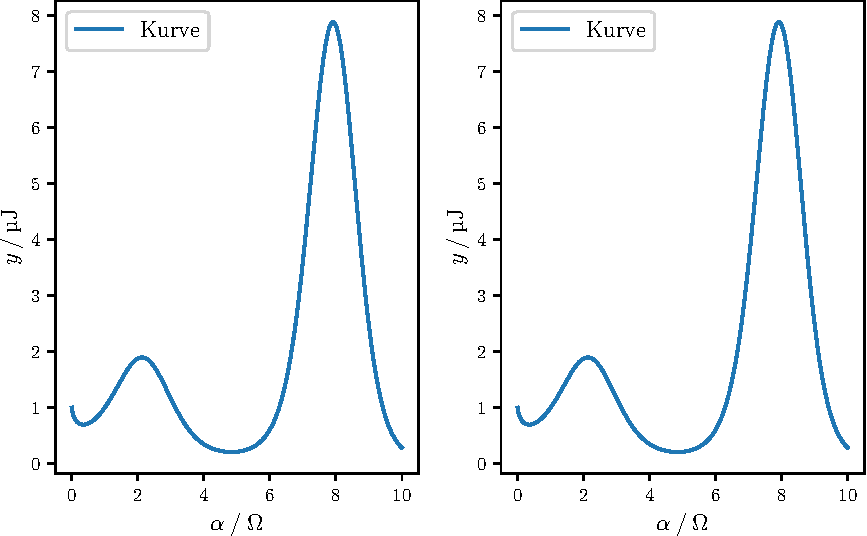
\includegraphics{plot.pdf}
%  \caption{Plot.}
%  \label{fig:plot}
%\end{figure}